%=======================================================================
% 流水线自测用中文版前言（不是真实报告）
% 编译：在 selftest/zh/ 下执行 xelatex 两遍
%=======================================================================
\documentclass[11pt,openany]{ctexart}

% =====================================================================
%  preamble-common.tex
%  Shared preamble for the RetNet-272M technical report (Chinese and
%  English editions).  Build with XeLaTeX.
%
%  Typographic convention (deliberately plain, single column, as in a
%  conventional technical report):
%    * serif body text, no coloured display headings
%    * numbered tables and figures, each with a caption
%    * remarks set as an indented, labelled passage rather than a
%      coloured box
% =====================================================================

\usepackage{amsmath}
\usepackage{amssymb}
\usepackage{bm}

% ---------- layout ---------------------------------------------------
\usepackage[a4paper,top=2.5cm,bottom=2.5cm,left=2.4cm,right=2.4cm]{geometry}
\usepackage{fancyhdr}
\usepackage{titlesec}
\usepackage{enumitem}
\usepackage{booktabs}
\usepackage{array}
\usepackage{tabularx}
% A table taller than a page must be able to break across pages: an unbreakable
% `tabular` that large is shipped out past the paper edge (Overfull \vbox), and
% the part below the edge is what the reader loses.  `longtable` is used only
% for such tables (see mktex.render_table).
\usepackage{longtable}
\usepackage{ragged2e}
\usepackage{xcolor}
\usepackage{caption}
\usepackage{graphicx}

% ---------- code -----------------------------------------------------
\usepackage{listings}
\usepackage{newunicodechar}

% ---------- references ----------------------------------------------
\usepackage[hidelinks,bookmarksnumbered]{hyperref}
\usepackage{bookmark}

% ---------- colours (used sparingly: code and rules only) ------------
\definecolor{codebg}{RGB}{248,248,249}
\definecolor{codeframe}{RGB}{216,220,225}
\definecolor{codecomment}{RGB}{104,124,108}
\definecolor{codekeyword}{RGB}{0,80,150}
\definecolor{codestring}{RGB}{160,60,40}
\definecolor{rulecol}{RGB}{178,182,188}
\definecolor{headrule}{RGB}{40,48,60}

% ---------- spacing --------------------------------------------------
\linespread{1.04}
\setlength{\parskip}{0.30em}
\setlength{\parindent}{0pt}
\setlength{\abovedisplayskip}{6pt}
\setlength{\belowdisplayskip}{6pt}
\setlength{\abovedisplayshortskip}{4pt}
\setlength{\belowdisplayshortskip}{4pt}

% Mixed CJK / monospace prose has few hyphenation opportunities; give TeX
% more room to stretch instead of leaving overfull boxes.
\tolerance=3000
\emergencystretch=3em
\hyphenpenalty=50
\hbadness=10000

% ---------- headings: plain, black, not coloured ---------------------
\titleformat{\section}
  {\normalfont\large\bfseries}{\thesection}{0.7em}{}
\titleformat{\subsection}
  {\normalfont\normalsize\bfseries}{\thesubsection}{0.7em}{}
\titleformat{\subsubsection}
  {\normalfont\normalsize\itshape}{\thesubsubsection}{0.7em}{}
\titlespacing*{\section}{0pt}{1.5em}{0.55em}
\titlespacing*{\subsection}{0pt}{1.05em}{0.40em}
\titlespacing*{\subsubsection}{0pt}{0.85em}{0.30em}

% ---------- header / footer ------------------------------------------
\pagestyle{fancy}
\fancyhf{}
\renewcommand{\headrulewidth}{0pt}
\renewcommand{\footrulewidth}{0pt}
\fancyfoot[C]{\small\thepage}

% ---------- tables and figures ---------------------------------------
\renewcommand{\arraystretch}{1.18}
\setlength{\tabcolsep}{5pt}
\captionsetup{
  font=small,
  labelfont=bf,
  labelsep=period,
  justification=raggedright,
  singlelinecheck=false,
  skip=5pt,
}
\captionsetup[table]{position=top}
\captionsetup[figure]{position=bottom}

% A numbered table with its caption above, as in the reference report.
\newenvironment{reporttable}[1]
  {\begin{center}\small\captionof{table}{#1}}
  {\end{center}}
\newcommand{\tabnote}[1]{\par\vspace{2pt}{\footnotesize #1}}

% ---------- lists ----------------------------------------------------
\setlist[itemize]{topsep=0.25em,itemsep=0.12em,parsep=0.08em,leftmargin=1.5em}
\setlist[enumerate]{topsep=0.25em,itemsep=0.12em,parsep=0.08em,leftmargin=1.8em}

% ---------- inline code ----------------------------------------------
\newcommand{\code}[1]{\texttt{\small #1}}
\newcommand{\file}[1]{\texttt{\small #1}}

% ---------- code listings --------------------------------------------
\lstdefinestyle{report}{
  backgroundcolor=\color{codebg},
  basicstyle=\ttfamily\fontsize{8.1}{9.6}\selectfont,
  commentstyle=\color{codecomment}\itshape,
  keywordstyle=\color{codekeyword}\bfseries,
  stringstyle=\color{codestring},
  frame=single,
  rulecolor=\color{codeframe},
  framesep=5pt,
  framexleftmargin=5pt,
  xleftmargin=5pt,
  breaklines=true,
  breakatwhitespace=false,
  breakindent=1.2em,
  columns=fullflexible,
  keepspaces=true,
  showstringspaces=false,
  tabsize=4,
  aboveskip=0.6em,
  belowskip=0.6em,
  upquote=true,
  extendedchars=true,
  inputencoding=utf8,
  escapechar=|,
  texcl=false,
  literate=%
    {→}{{$\rightarrow$}}1
    {←}{{$\leftarrow$}}1
    {×}{{$\times$}}1
    {÷}{{$\div$}}1
    {≈}{{$\approx$}}1
    {≤}{{$\leq$}}1
    {≥}{{$\geq$}}1
    {≠}{{$\neq$}}1
    {µ}{{$\mu$}}1
    {γ}{{$\gamma$}}1
    {Δ}{{$\Delta$}}1
    {σ}{{$\sigma$}}1
    {τ}{{$\tau$}}1
    {Σ}{{$\Sigma$}}1
    {√}{{$\surd$}}1
    {·}{{$\cdot$}}1
    {−}{{$-$}}1
    {∈}{{$\in$}}1
    {±}{{$\pm$}}1
    {∞}{{$\infty$}}1
    {❌}{{$\times$}}1
    {✅}{{$\checkmark$}}1
    {⚠}{{!}}1
}
\lstset{style=report}

% `listings` ships no PowerShell dialect; define just enough to colour it.
\lstdefinelanguage{PowerShell}{
  morekeywords={if,else,elseif,foreach,for,while,function,param,return,
    try,catch,finally,switch,break,continue,throw,in,not,and,or},
  sensitive=false,
  morecomment=[l]{\#},
  morestring=[b]",
  morestring=[b]',
}
\lstdefinelanguage{text}{}

% ---------- remarks --------------------------------------------------
% The source uses block quotes for asides.  They are set as an indented
% passage introduced by "Note." rather than as a coloured box.
\newenvironment{notebox}
  {\par\vspace{0.35em}%
   \begin{list}{}{%
     \setlength{\leftmargin}{1.5em}\setlength{\rightmargin}{0.4em}%
     \setlength{\topsep}{0pt}\setlength{\parskip}{0.25em}%
     \setlength{\parsep}{0.25em}\setlength{\itemsep}{0pt}%
     \setlength{\listparindent}{0pt}}%
   \item\relax\textbf{Note.}\ \ignorespaces}
  {\end{list}\vspace{0.15em}}

% ---------- rule -----------------------------------------------------
\newcommand{\reportrule}{\par\vspace{0.5em}{\color{rulecol}\hrule height 0.4pt}\vspace{0.7em}\par}

% ---------- appendices -----------------------------------------------
% The source writes the appendix titles with their letter already in the
% text ("Appendix A: Reproduction"), so the appendix section counter prints
% the letter and the *headings* of the back matter use a second counter that
% renumbers (Reference Reliability Note, References).
\newcounter{backmatter}
\newcommand{\startappendix}{%
  \clearpage
  \setcounter{section}{0}%
  \setcounter{backmatter}{0}%
  \renewcommand{\thesection}{\Alph{section}.}%
  % subsections are numbered against the appendix letter, so pin the format
  % explicitly: leaving \thesubsection as \thesection.\arabic{subsection}
  % would print `B..1' because \thesection already ends in a period.
  \renewcommand{\thesubsection}{\Alph{section}.\arabic{subsection}}%
}
\newcommand{\backmattersection}[1]{%
  \refstepcounter{backmatter}%
  \section*{\arabic{backmatter}.\quad #1}%
  \addcontentsline{toc}{section}{\protect\numberline{\arabic{backmatter}.}#1}%
}


% 中文字体：正文宋体 / 强调黑体 / 引用楷体 / 等宽仿宋
\setCJKmainfont{SimSun}[BoldFont=SimHei,ItalicFont=KaiTi]
\setCJKsansfont{Microsoft YaHei}
\setCJKmonofont{FangSong}

\hypersetup{
  pdftitle  = {流水线自测占位报告},
  pdfauthor = {RetNet 项目组},
  pdfsubject= {LaTeX 流水线自测},
}

\begin{document}


%=======================================================================
% 流水线自测用中文版标题页 — 由 mktex.py 插在正文之前
% 摘要与目录由构建器紧随其后插入（front matter）
%=======================================================================
\thispagestyle{empty}

\begin{center}
\vspace*{3.2cm}

{\LARGE\bfseries 流水线自测占位报告}

\vspace{0.55cm}

{\large RetNet-0.5B LaTeX Pipeline Self-Test}

\vspace{1.1cm}

{\normalsize RetNet 项目组}

\vspace{0.25cm}

{\small\itshape 2026-10-13}

\vspace{2.2cm}

\begin{minipage}{0.80\textwidth}
\centering\small
\begin{tabular}{@{}rl@{}}
\toprule
用途 & 验证「中文单语 md → 中文版 PDF」与「英文补充稿 → 英文版 PDF」\\
模型 & 504.18\,M 参数，20 层，1408 维，22 头（占位引用）\\
数据 & 552.33\,M token $\times$ 3 epoch（占位引用）\\
\bottomrule
\end{tabular}
\end{minipage}

\vfill

{\small\itshape 本 PDF 是自测产物，不是交付报告。}

\vspace{1.2cm}
\end{center}

\clearpage


\section*{摘要}

\addcontentsline{toc}{section}{摘要}

本占位稿由 \code{mktex\allowbreak{}.py} 的 \code{selftest} 配置读入：中文版直接取本文件正文，英文版全文来自 \code{selftest\allowbreak{}/en\allowbreak{}/\allowbreak{}\_supplement\allowbreak{}.tex}。这一节同时验证「摘要由 Markdown 提供、排在目录之前、标题进目录但不编号」 的处理方式；若把 \code{\allowbreak{}\#\allowbreak{}\# 摘要} 写成 \code{\allowbreak{}\#} 之外的其它层级，构建器会打印一条 front-matter 警告。

\renewcommand{\contentsname}{目录}
\tableofcontents

\clearpage

\section{引言}

这一段验证中文正文的行内渲染：行内代码 \code{RETNET\allowbreak{}\_FAST\allowbreak{}\_CHUNKWISE=1}、加粗 \textbf{重点结论}、 链接 \href{README.md}{README}、以及行内数学 $d_{\mathrm{model}} = 1408$。 换行与长代码 \code{\allowbreak{}-\allowbreak{}-resume checkpoints\allowbreak{}/retnet\allowbreak{}\_500m\allowbreak{}\_v15b\allowbreak{}/checkpoint\allowbreak{}-67390} 应当正常断行。

\subsection{列表与引用}

\begin{itemize}
  \item 第一项：验证无序列表；
\end{itemize}
\begin{itemize}
  \item 第二项：验证嵌套列表：
\end{itemize}

\begin{enumerate}
  \item 嵌套有序项一；
  \item 嵌套有序项二。
\end{enumerate}

\begin{notebox}
这一段是引用块，应当渲染成以 Note. 起头的缩进段落，而不是灰底框。
\end{notebox}

\section{架构}

\subsection{模型配置表}

\begin{center}
\small
\captionof{table}{数据构成实测}
\begin{tabular}{>{\RaggedRight\arraybackslash}p{114.0pt}>{\RaggedRight\arraybackslash}p{91.0pt}>{\RaggedRight\arraybackslash}p{230.0pt}}
\toprule
\textbf{项} & \textbf{值} & \textbf{出处} \\
\midrule
参数量 & 504,179,896 & \code{checkpoints\allowbreak{}/retnet\allowbreak{}\_500m\allowbreak{}\_v15b\allowbreak{}\_ep3\allowbreak{}/model\allowbreak{}.safetensors} \\
d\allowbreak{}\_model / layers / heads & 1408 / 20 / 22 & \code{config\allowbreak{}.json} \\
存储精度 & \code{float32}（训练 bf16） & \code{config\allowbreak{}.json} \\
\bottomrule
\end{tabular}
\end{center}

\subsection{代码块}

\begin{lstlisting}[language=Python]
def retention(x, gamma):
    """自测用代码块：验证 listings 样式与中文注释。"""
    return x * gamma
\end{lstlisting}

\subsection{热重启代价}

\begin{figure}[htbp]
\centering
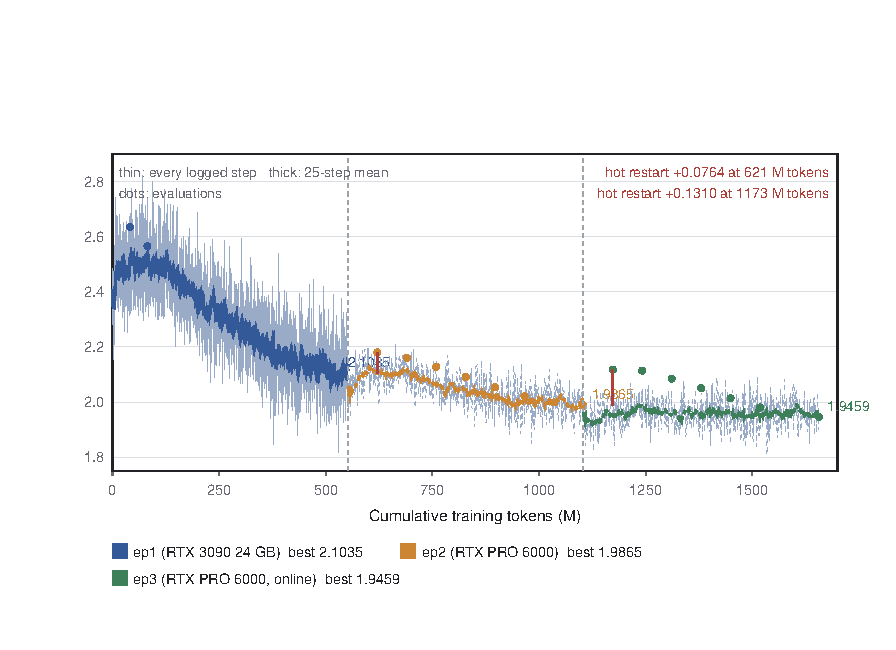
\includegraphics[width=\linewidth]{../../figures/fig-0p5b-loss}
\caption{三段训练的验证 loss：每段都重启一条完整 cosine，热重启后首个评测点高于上一段最优，差值见图中标注。数据源为三段 \code{trainer\_state.json}。}
\label{fig:fig-0p5b-loss}
\end{figure}

\begin{figure}[htbp]
\centering
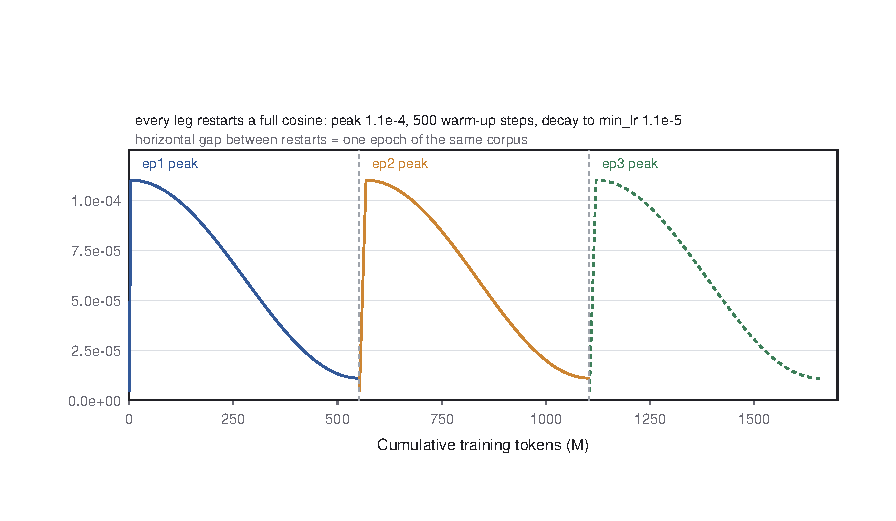
\includegraphics[width=\linewidth]{../../figures/fig-0p5b-lr}
\caption{三段的学习率轨迹：每段都重启一条完整 cosine（峰值 $1.1\times10^{-4}$、warm-up 500 步、衰减到 \code{min\_lr} $1.1\times10^{-5}$），段间不接续。数据源同上一张图。}
\label{fig:fig-0p5b-lr}
\end{figure}

\begin{center}
\small
\captionof{table}{热重启的代价}
\begin{tabular}{lrrr}
\toprule
\textbf{衔接} & \textbf{上一段最优} & \textbf{下一段首次评测} & \textbf{差} \\
\midrule
ep1 $\rightarrow$ ep2 & 2.1035 @65000 & 2.1800 @2106 & +0.0764 \\
ep2 $\rightarrow$ ep3 & 1.9865 @16848 & 2.1174 @2106 & +0.1310 \\
\bottomrule
\end{tabular}
\end{center}

三段训练共 1,656,340,480 token，token/参数 = 3.285。

\backmattersection{参考文献}\label{sec:refs}

\begin{enumerate}
  \item Retentive Network: A Successor to Transformer for Large Language Models. arXiv:2307.08621.
\end{enumerate}
\begin{enumerate}
  \item Gated Linear Attention Transformers with Hardware-Efficient Training. arXiv:2312.06635.
\end{enumerate}

\startappendix

\section{附录 A：复现命令}

\begin{lstlisting}[language=PowerShell]
python makefigs.py
python mktex.py --report selftest
\end{lstlisting}

\end{document}
